\section{First test in oven}

The first trial in the oven took place 2017-03-28 at Mefos in Lule\r{a}. The data communication worked during the time in the oven, where the data could be followed using Electrotech's radio antenna and serial communication.

When heating up the oven, it didn't reach its expected temperature in time. This caused some delays and the sensor was then placed in the oven 3 hours later than planned. This gave us the opportunity to do some fault searching for the sensor, which stopped working sometimes for unknown reasons. However what seemed like a pattern was that the sensor system started to fail during the heat up process after it entered sleep mode.


Because of this, the sensor was heated up with a separate voltage cube and made sure it gave some valid data before placing it into the oven and the system was never reentering sleep mode after this heat up process.


Just the tip of the sensor was pointing out from the isolation material and had direct contact with the oven's environment. It took about 10-15 minutes for the sensor to reach its operating temperature and this time could be decreased by either expose a bigger part of the sensor to the oven or preheat the sensor with a gas burned or similar. However, by exposing a bigger part of the sensor to the oven, it will most probably decrease its lifetime.

\begin{figure}
    \centering
    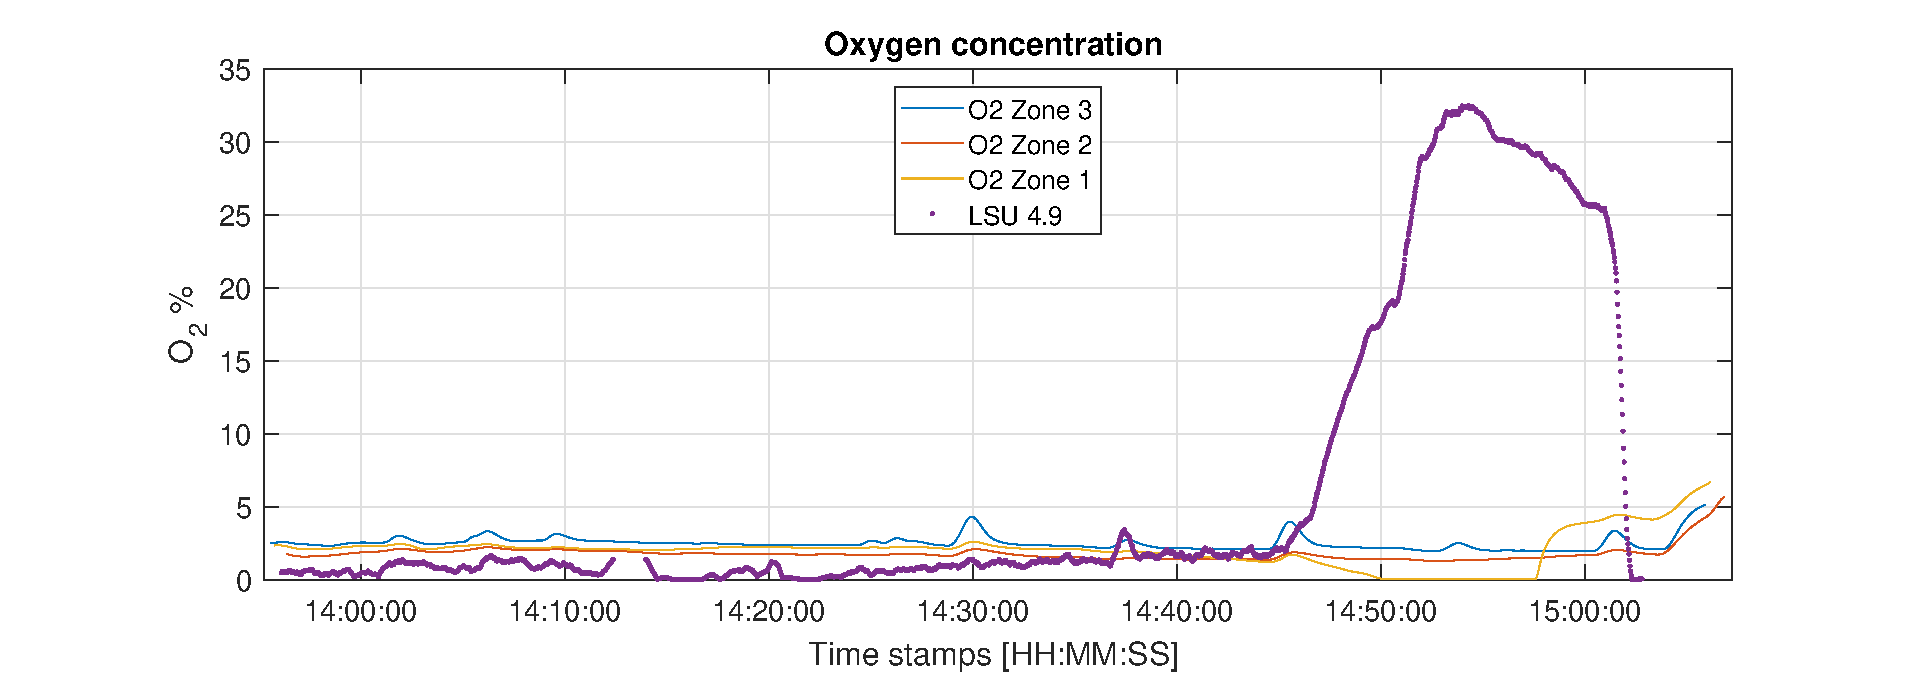
\includegraphics[width=\textwidth]{Chapter4/Figures/syre_dots.eps}
    \caption{The oxygen level during the test.}
    \label{fig:syre_dots}
\end{figure}

\subsection{Measurements during the first test.}

Figure \ref{fig:syre_dots} shows the oxygen values measured by the lambda sensor during its time in the oven. There are also three lines with reference measurements. Exactly what time the sensor went from one zone to another is hard to tell. But the time in each zone was the same, where it started in zone 1. There is also a gap with no data in this graph. This is due to unreliable data and therefore neglected. The oxygen calculations are not correct when the lambda value is below 1, which represent a negative current on the pumping current, and that most probably what happened.

In figure \ref{fig:nernst_both} there are two lines made by the same data. Both lines show the voltage drop over the nernst cell during the time in the oven, where the orange line is mean value by nearby data. This voltage is supposed to be 450 mV and from the beginning it was below this limit. This time was before the sensor reached its operating temperature.


\begin{figure}
    \centering
    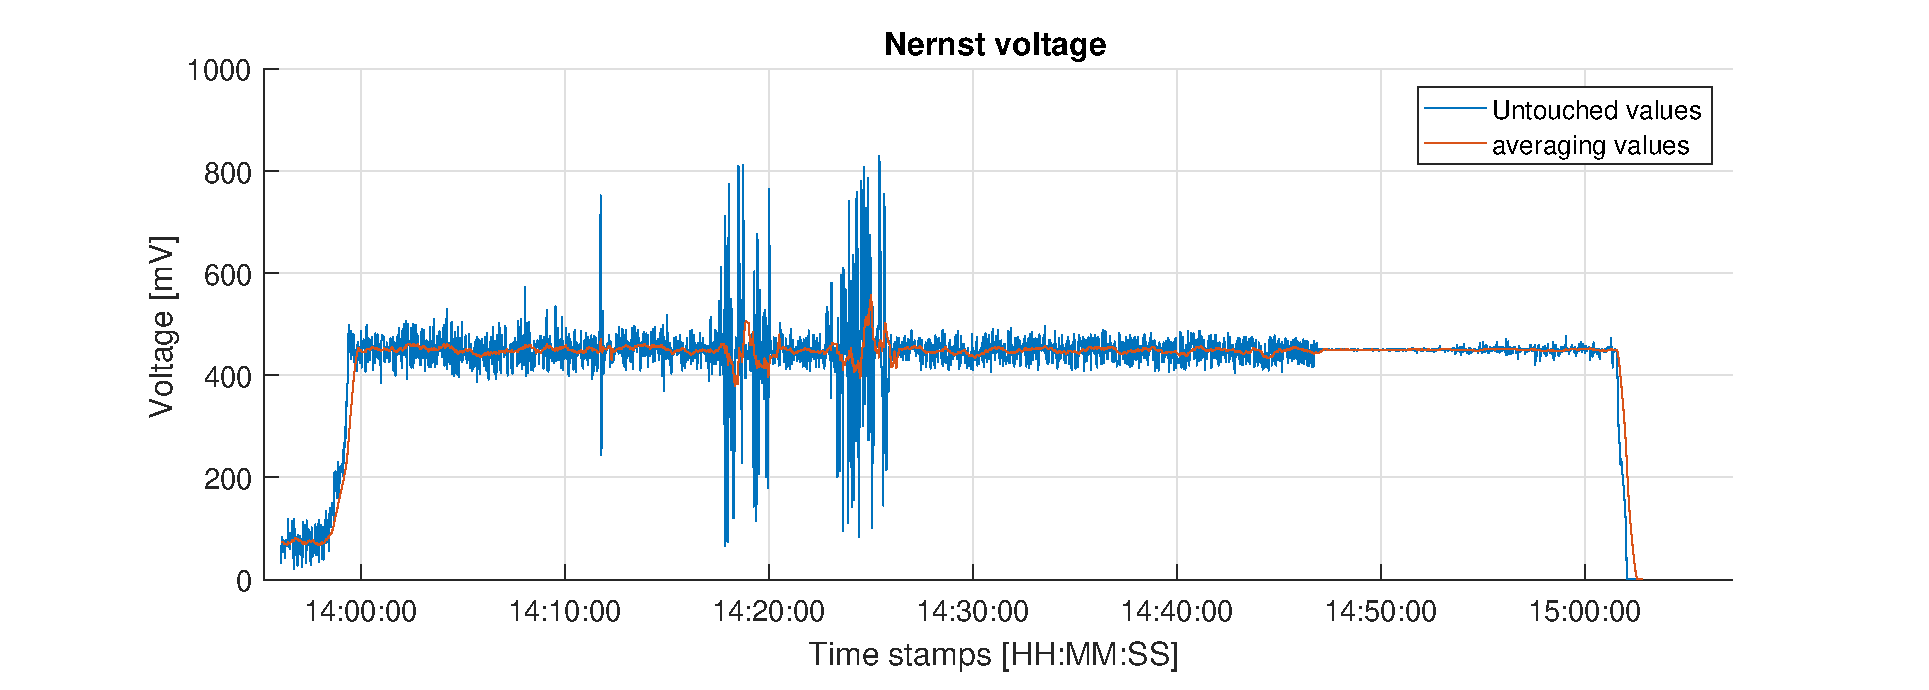
\includegraphics[width=\textwidth]{Chapter4/Figures/nernst_both.eps}
    \caption{The voltage over the nernst cell during the test.}
    \label{fig:nernst_both}
\end{figure}

Figure \ref{fig:temperature_both} also have two lines done with same data. The blue line is untouched values and the orange is the mean value of nearby measurements. Figure \ref{fig:temperature_both}, shows the temperature of the sensor during its time in the oven and this temperature is calculated by measuring the resistance over the nernst cell.





\begin{figure}
    \centering
    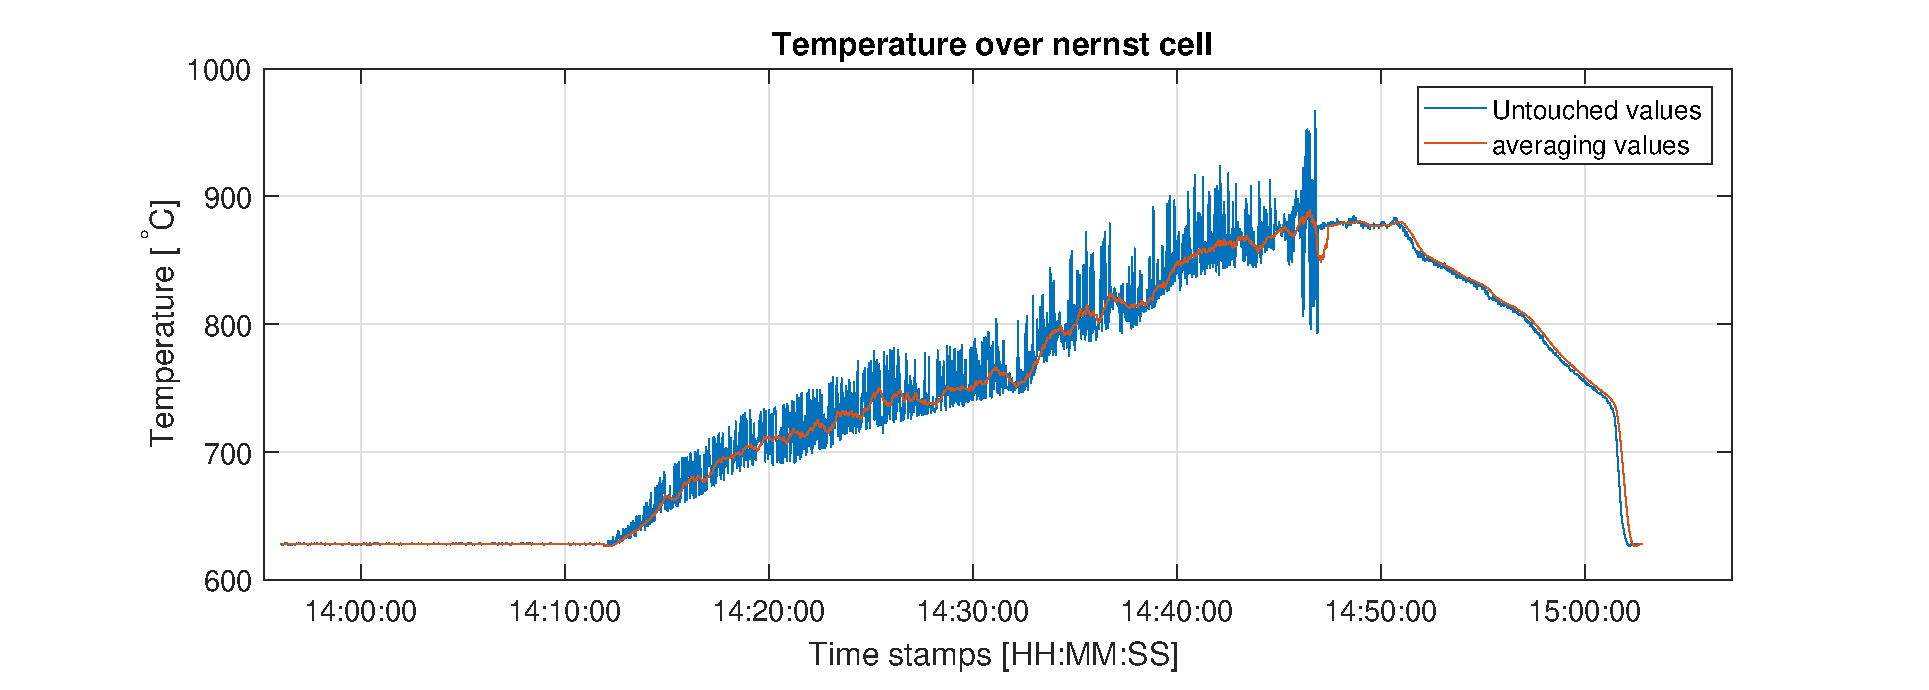
\includegraphics[width=\textwidth]{Chapter4/Figures/temperature_both.eps}
    \caption{The PWM temperature measurement during the test.}
    \label{fig:temperature_both}
\end{figure}


\subsection{Day after test}

The day after the first test was performed, the lambda sensor with its electronics was collected and brought back to \ac{ltu}. Because the water only reached 70 degrees, the electronics and the mechanical design still looked to be in good shape. There was still some power in the batteries and Electrotech's radio system still sent data, which were collected by the antenna. The sensor was then heated up with a power supply and when it reached its operating temperature, it started to send correct oxygen concentration for the room.

So the system did survive the 2 hours in the oven and could then be re-used. At least the electronics could be re-used, without any risk. But how much the time in the oven shortened the lambda sensor's lifetime is hard to tell though.



%\section{Small tests at Mefos}
\section{Tests in small oven at Mefos}

\subsection{First test 20170412}

This test was done in a small oven heated up to 1200 $^\circ$C. The lambda sensor was then put in the oven through a small hole and it reached its operating temperature fast. The temperature of the sensor kept increasing until it broke however, so this sensor only managed to give data for a short amount of time before it broke down.

Another lambda sensor then replaced this sensor. The resistance on the electronics was calibrated for the first lambda sensor, so the values of the second sensor were a bit shifted. This sensor was not placed as deep in the oven as the first sensor. So this time the sensor survived much better and gave valid data. The values seemed to have an offset compared to the reference measurement and it was a bit noisy as well. If the condition in the oven was changed, the lambda sensor and reference sensor changed in the same way. But it was still an offset error by a factor of about 3.

After some changes of the oxygen levels, it was a plan to change the regulator of the nernst voltage a bit and the programmer was placed to the electronics. Immediately when the programmer was connected both the oxygen and nernst measurement become more stable. But it still had an offset, which seemed to change a bit.




\subsection{Second test 20170420}

The changes in this test compared to the first test in a small oven, were that the position of the reference measurement for the oxygen was changed and the controller for the pump current was slightly changed.

The previous time, the reference measurement was placed at the top corner of the oven. This was a bigger hole compared to the one where the lambda sensor was placed. This measurement was moved to the same hole as the lambda sensor this time and it made a big difference in the oxygen concentration for the reference measurement. This hole is placed in the middle of a wall of the oven.

\begin{figure}
    \centering
    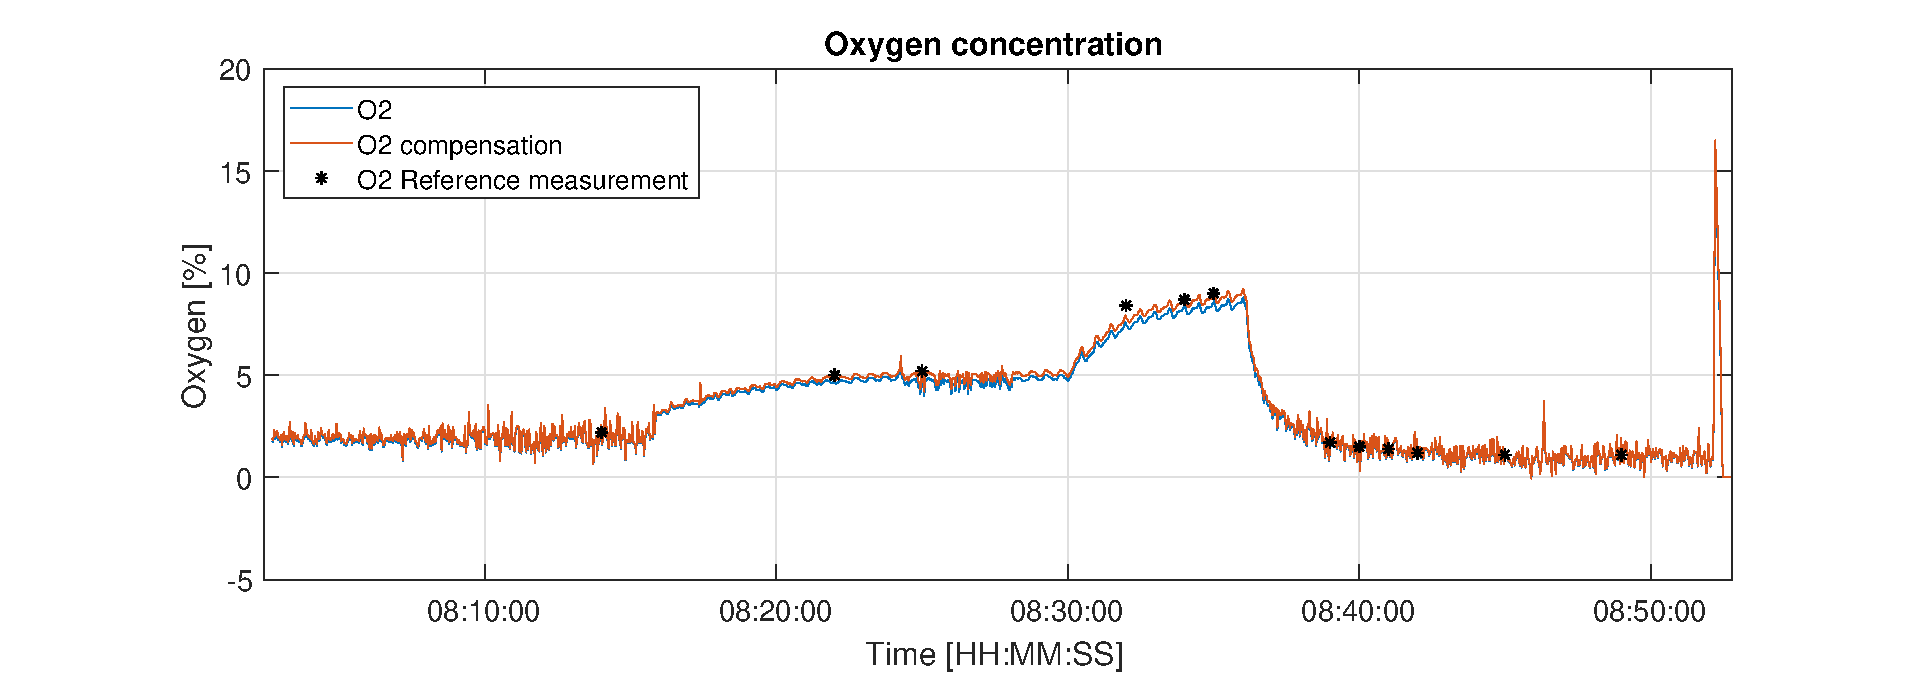
\includegraphics[width = \textwidth]{Chapter4/Figures/oxygen_second_small.eps}
    \caption{Oxygen measurement in small oven with reference points.}
    \label{fig:oxygen_second_small}
\end{figure}

In figure \ref{fig:oxygen_second_small} and \ref{fig:nernst_second_small} one can see that the measurements are clearly more stable at two time intervals. During these intervals, the sensor was also heated from a voltage cube and not only from the heat produced by the oven.

The reference measurement in figure \ref{fig:oxygen_second_small} was performed by a separate unit, which didn't log the measurement data and test points was then noted now and then manually.

\begin{figure}
    \centering
    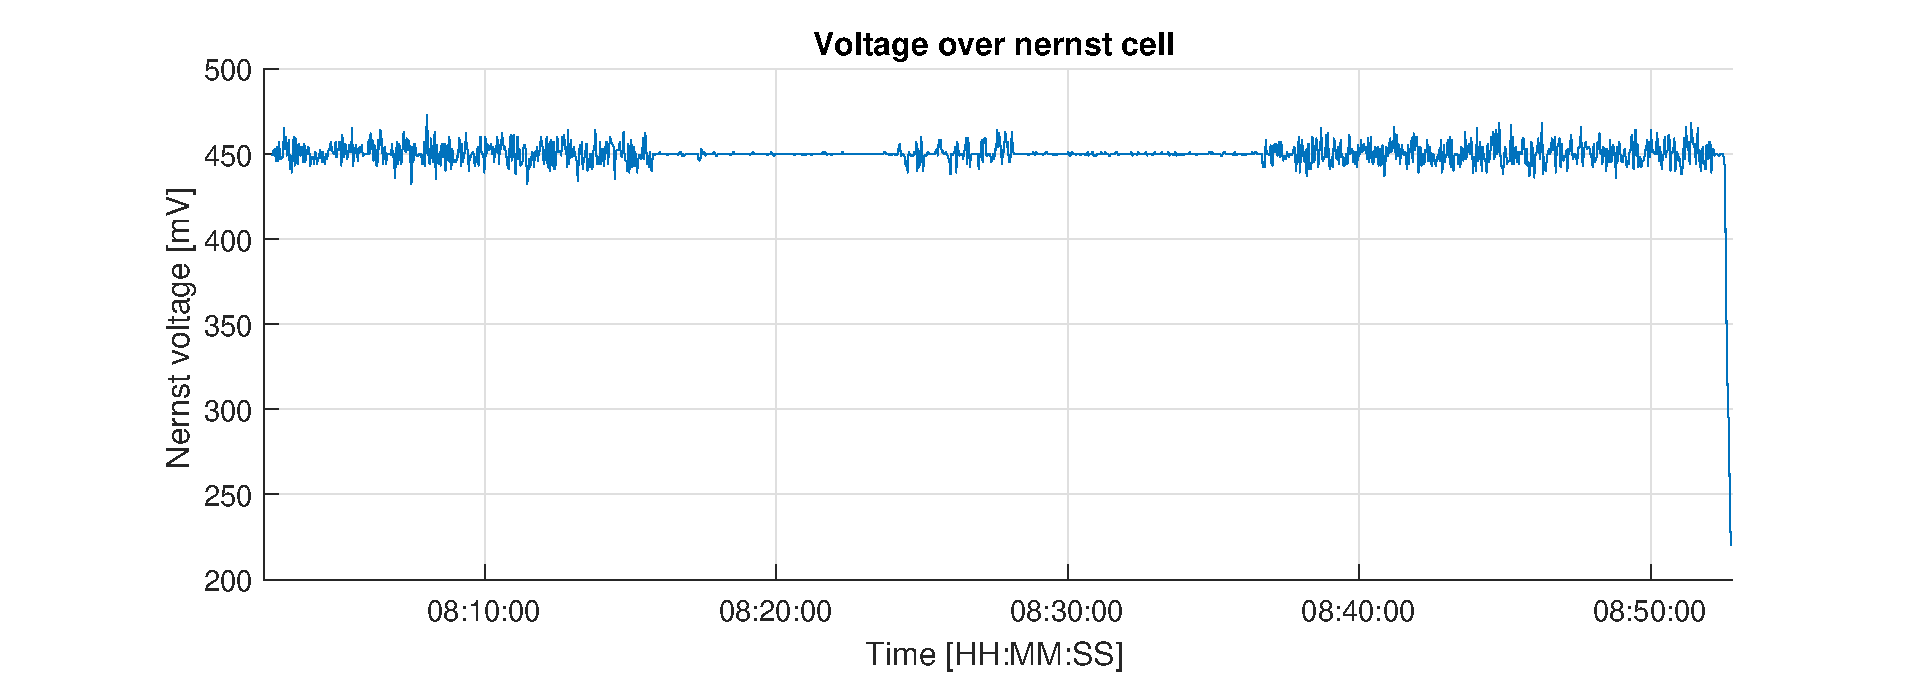
\includegraphics[width = \textwidth]{Chapter4/Figures/nernst_second_small.eps}
    \caption{Voltage drop over nernst cell at the test in a small oven.}
    \label{fig:nernst_second_small}
\end{figure}

The temperature measurements in figure~\ref{fig:temperature_second_small} are done by measuring the resistance over the nernst cell. These temperature measurements are valid from approximate 630 $^\circ$C and above. The actual temperature is most likely below this temperature when the measurement is stable at 630 $^\circ$C for longer times.


\begin{figure}
    \centering
    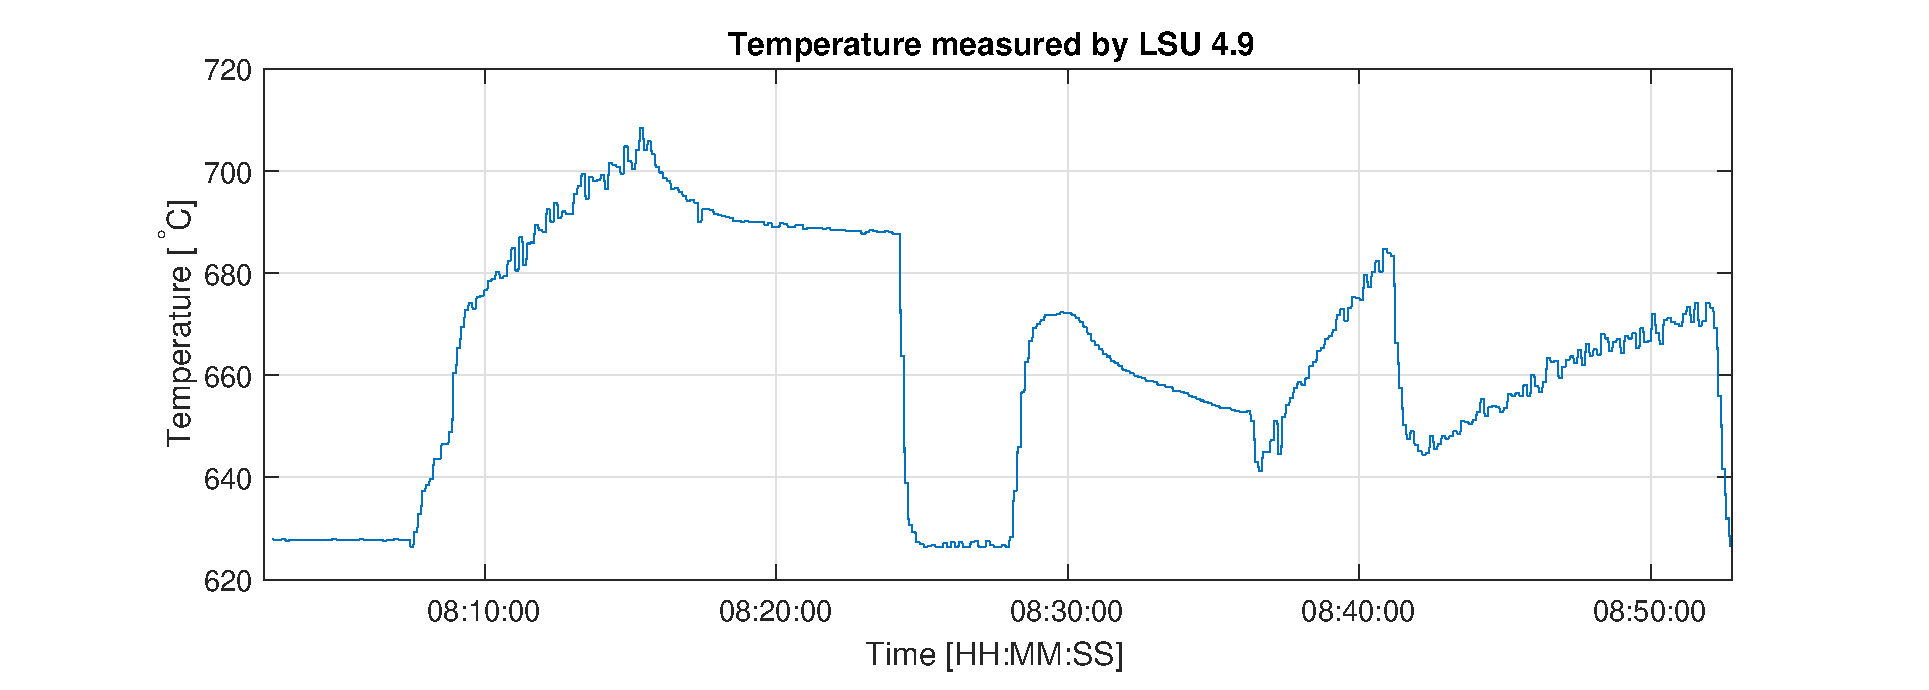
\includegraphics[width = \textwidth]{Chapter4/Figures/temperature_second_small.eps}
    \caption{Temperature measurement at sensor element.}
    \label{fig:temperature_second_small}
\end{figure}

